\section{Experimental results}\label{sec:results}
\graphicspath{{./img/}}

To give comparative results on the quality of the initialisation processes
considered in this work, four well-known, categorical, labelled datasets ---
breast cancer, mushroom, nursery, and soybean (large) --- will be clustered by
the \(k\)-modes algorithm with each of the initialisation processes. These
datasets have been chosen to fall in line with the established literature, and
for their relative sizes and complexities. Each dataset is openly available
under the UCI Machine Learning Repository~\cite{Dua2019}, and their
characteristics are summarised in Table~\ref{tab:dataset_summary}. For the
purposes of this analysis, incomplete instances (i.e.\ where data is missing)
are excluded and the remaining dataset characteristics are reported as
`adjusted'.

\begin{table}[htbp]
    \resizebox{\textwidth}{!}{%
        \begin{tabular}{lrrrlrr}
\toprule
{} &  No. rows &  No. cols &  No. classes &  Missing values &  Adjusted no. rows &  Adjusted no. classes \\
\midrule
Breast cancer &       699 &        10 &            2 &            True &                683 &                     2 \\
Mushroom      &      8124 &        22 &            2 &            True &               5644 &                     2 \\
Soybean       &       307 &        35 &           19 &            True &                266 &                    15 \\
Nursery       &     12960 &         8 &            5 &           False &              12960 &                     5 \\
\bottomrule
\end{tabular}

    }\caption{A summary of the benchmark datasets.}\label{tab:dataset_summary}
\end{table}

All of the source code used to produce the results and data in this analysis ---
including the datasets investigated in Section~\ref{subsec:artificial} --- are
archived at DOI. In addition to this, the implementation of the \(k\)-modes
algorithm and its initialisations is available under
DOI~\href{https://doi.org/10.5281/zenodo.3638035}{10.5281/zenodo.3638035}.

This analysis does not consider evaluative metrics related to classification
such as accuracy, recall or precision as is commonly done~\cite{%
    Arthur2007,Cao2009,Cao2012,Huang1998,%
    Ng2007,Olaode2014,Schaeffer2007,Sharma2015%
}. Instead, only internal measures are considered such as the cost function
defined in~\eqref{eq:cost}. This metric is label-invariant and its values are
comparable across the different initialisation methods. Furthermore, the effect
of each initialisation method on the initial and final clusterings can be
captured with the cost function. An additional, and often useful, metric is the
silhouette coefficient. This measures the ratio between the intra-cluster
cohesion and inter-cluster separation of a particular clustering. Therefore, it
could be used in a similar way to reveal the effect of each initialisation
method at the beginning and end of a run of \(k\)-modes. Unfortunately, this
metric loses its intuition under the distance measure employed here and is
omitted. The remaining performance measures used are the number of iterations
for the \(k\)-modes algorithm to terminate and the time taken to terminate in
seconds.

The final piece of information required in this analysis is a choice for \(k\)
for each dataset. An immediate choice is the number of classes that are present
in a dataset but this is not necessarily an appropriate choice since the classes
may not be representative of true clusters~\cite{Memoli2011}. However, this
analysis will consider this case as there may be practical reasons to limit the
value of \(k\). The other strategy for choosing \(k\) considered in this work
uses the knee point detection algorithm introduced in~\cite{Satopaa2011}. This
strategy was chosen over other popular methods such as the `elbow' method as its
results are definitive.

The knee point detection algorithm was employed over values of \(k\) from 2 up
to \(\lfloor\sqrt N\rfloor\) for each dataset. The number of clusters determined
by this strategy is reported in the final column of
Table~\ref{tab:dataset_summary}.


\subsection{Using knee point detection algorithm for \(k\)}\label{subsec:knee}

Tables~\ref{tab:breast_cancer_knee}---\ref{tab:soybean_knee}
summarise the results of each initialisation method on the benchmark datasets
where the number of clusters has been determined by the knee point detection
algorithm. Each column shows the mean value of each metric and its standard
deviation in parentheses over 250
independent
repetitions of the \(k\)-modes algorithm.

\begin{table}[htbp]
    \centering
    \resizebox{\tablewidth}{!}{%
        \begin{tabular}{lllll}
\toprule
{} &       Initial cost &        Final cost & No. iterations &          Time \\
\midrule
Cao      &    3118.00 (0.000) &   2774.00 (0.000) &   4.00 (0.000) &  0.30 (0.012) \\
Huang    &  2856.50 (104.245) &  2748.83 (64.514) &   2.68 (0.817) &  0.22 (0.046) \\
Matching &  2870.11 (101.869) &  2752.59 (52.387) &   2.72 (0.760) &  0.16 (0.021) \\
\bottomrule
\end{tabular}

    }
    \captionof{table}{Summative metric results for the breast cancer dataset
    with \(k=8\).}\label{tab:breast_cancer_knee}\vspace{20pt}

    \resizebox{\tablewidth}{!}{%
        \begin{tabular}{lllll}
\toprule
{} &         Initial cost &          Final cost & No. iterations &          Time \\
\midrule
Cao      &     20381.00 (0.000) &    20376.00 (0.000) &   2.00 (0.000) &  4.68 (0.205) \\
Huang    &  23027.24 (1209.753) &  21869.06 (747.766) &   2.90 (0.934) &  5.11 (1.138) \\
Matching &  23279.36 (1498.324) &  21855.50 (751.641) &   3.02 (0.936) &  2.77 (0.325) \\
\bottomrule
\end{tabular}

    }
    \captionof{table}{Summative metric results for the mushroom dataset with
    \(k=17\).}\label{tab:mushroom_knee}\vspace{20pt}

    \resizebox{\tablewidth}{!}{%
        \begin{tabular}{lllll}
\toprule
{} &        Initial cost &          Final cost & No. iterations &          Time \\
\midrule
Cao      &    35544.00 (0.000) &    35544.00 (0.000) &   1.00 (0.000) &  4.98 (0.152) \\
Huang    &  37535.06 (372.596) &  37535.06 (372.596) &   1.00 (0.000) &  3.58 (0.121) \\
Matching &  37484.29 (327.467) &  37484.29 (327.467) &   1.00 (0.000) &  3.14 (0.141) \\
\bottomrule
\end{tabular}

    }
    \captionof{table}{Summative metric results for the nursery dataset with
    \(k=23\).}\label{tab:nursery_knee}\vspace{20pt}

    \resizebox{\tablewidth}{!}{%
        \begin{tabular}{lllll}
\toprule
{} &      Initial cost &        Final cost & No. iterations &          Time \\
\midrule
Cao      &   1654.00 (0.000) &   1585.00 (0.000) &   4.00 (0.000) &  0.28 (0.014) \\
Huang    &  1829.31 (92.308) &  1708.55 (69.740) &   3.58 (1.019) &  0.28 (0.063) \\
Matching &  1827.76 (86.852) &  1711.49 (73.319) &   3.42 (0.963) &  0.17 (0.022) \\
\bottomrule
\end{tabular}

    }
    \captionof{table}{Summative metric results for the soybean dataset with
    \(k=8\).}\label{tab:soybean_knee}
\end{table}

By examining these tables it would seem that the proposed method and Huang's
method are comparable across the board --- although the proposed method is
faster despite taking more iterations in general which may relate to a more
intuitive initialisation. More importantly though, it appears that Cao's method
performs the best out of the three initialisation methods: in terms of initial
and final costs Cao's method improves, on average, by roughly 10 percent against
the next best method for the three datasets that it succeeds with; the number of
iterations is comparable; and the computation time is substantially less than
the other two considering it is a deterministic method and need only be run once
to achieve this performance.

However, in the \(k\)-means paradigm, a particular clustering is selected based
on it having the minimum final cost over a number of runs of the algorithm ---
not the mean --- and while Cao's method is very reliable, in that there is no
variation at all, it does not always produce the best clustering possible. There
is a trade-off to be made between computational time and performance here. In
order to gain more insight into the performance of each method, less granular
analysis is required.
Figures~\ref{fig:breast_cancer_knee}---\ref{fig:soybean_knee} display the
cost function results for each dataset in the form of a scatter plot and two
empirical cumulative density function (CDF) plots, highlighting the breadth and
depth of the behaviours exhibited by each initialisation method.

Looking at Figure~\ref{fig:breast_cancer_knee} it is clear that in terms of
final cost Cao's method is middling when compared to the other methods. This
was apparent from Table~\ref{tab:breast_cancer_knee} and, indeed, Huang's and
the proposed method are both very comparable when looking at the main body of
the results. However, since the criterion for the best clustering (in practical
terms) is having the minimum final cost, it is evident that the proposed method
is superior; that the method produces clusterings with a larger cost
range (indicated by the trailing right-hand side of each CDF plot) is irrelevant
for the same reason.

This pattern of largely similar behaviour between Huang's and the proposed
method is apparent in each of the figures here, and in each case the proposed
method outperforms Huang's. In fact, in all cases except for the nursery
dataset, the proposed method achieves the lowest final cost of all the methods
and, as such, performs the best in practical terms on these particular datasets.

In the case of the nursery dataset, Cao's method is unquestionably the best
performing initialisation method. It should be noted that none of the
methods were able to find an initial clustering that could be improved on, and
that this dataset exactly describes the entire attribute space in which it
exists. This property could be why the other methods fall behind Cao's so
decisively in that Cao's method is able to definitively choose the \(k\) most
dense-whilst-separated points from the attribute space as the initial cluster
centres whereas the other two methods are in essence randomly sampling from this
space. That each initial solution in these repetitions is locally optimal
remains a mystery.

\begin{figure}
    \begin{subfigure}{.5\textwidth}
        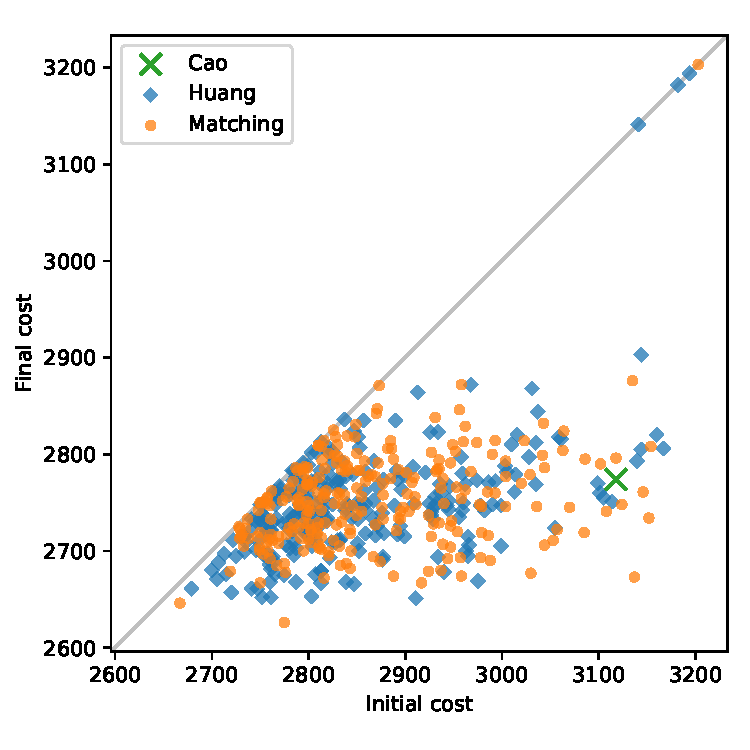
\includegraphics[width=\linewidth]{Fig1a.pdf}
        \caption{Scatter plot of initial and final costs.}
    \end{subfigure}
    \hfill%
    \begin{subfigure}{.5\textwidth}
        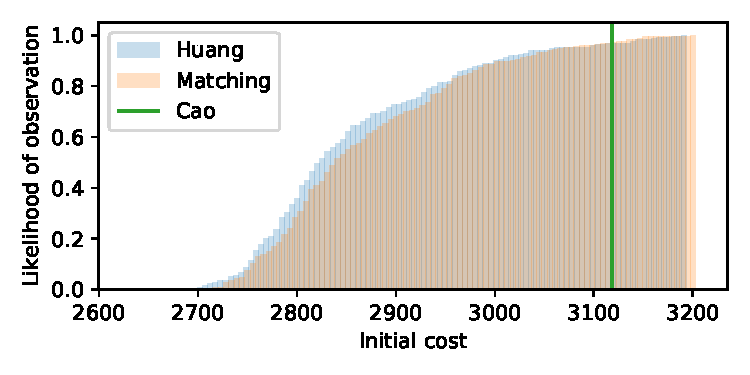
\includegraphics[width=\linewidth]{Fig1b1.pdf}

        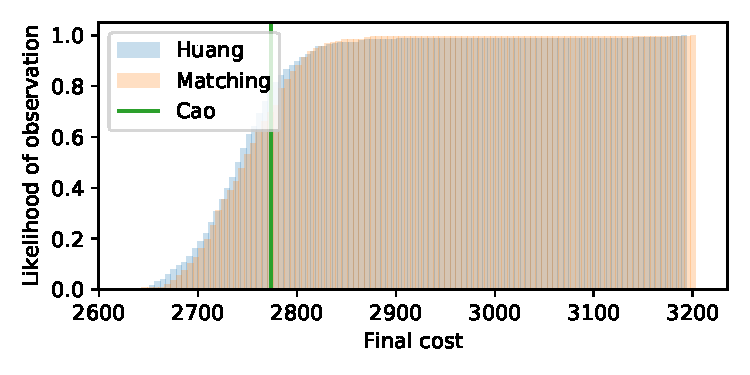
\includegraphics[width=\linewidth]{Fig1b2.pdf}
        \caption{Empirical CDF plots for initial (top) and final (bottom)
                 costs.}
    \end{subfigure}
    \caption{Summative plots for the breast cancer dataset with \(k=8\).}%
    \label{fig:breast_cancer_knee}
\end{figure}

\begin{figure}
    \begin{subfigure}{.5\textwidth}
        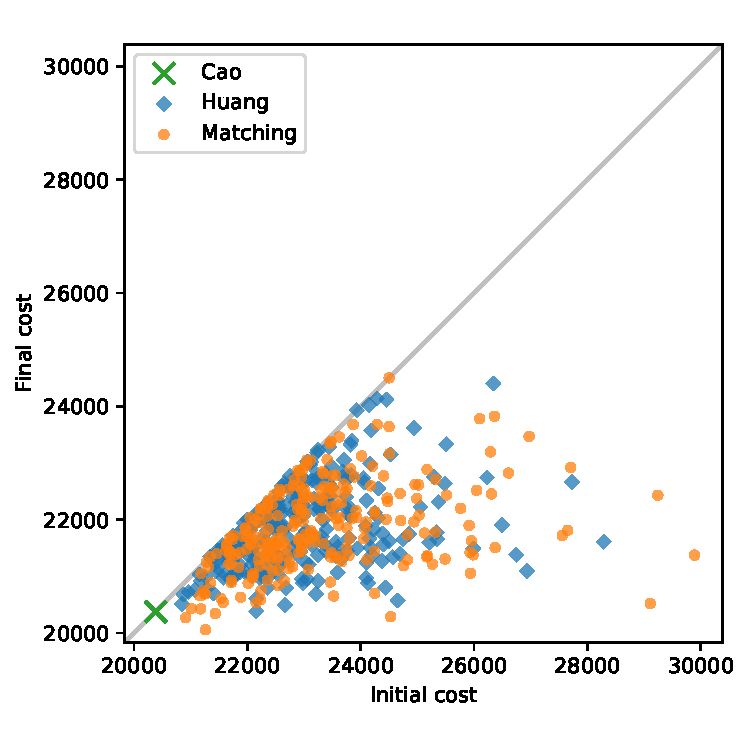
\includegraphics[width=\linewidth]{Fig2a.pdf}
        \caption{Scatter plot of initial and final costs.}
    \end{subfigure}
    \hfill%
    \begin{subfigure}{.5\textwidth}
        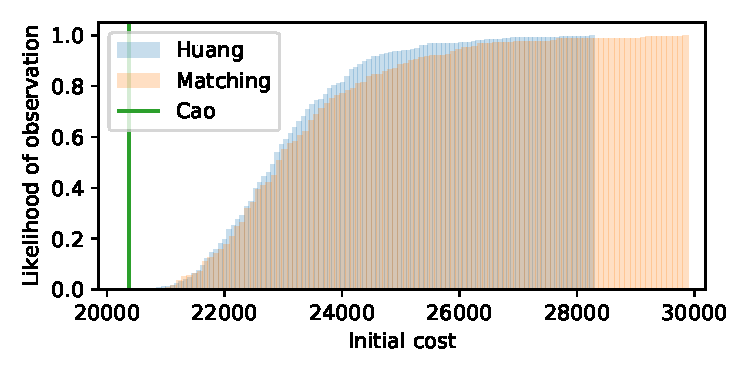
\includegraphics[width=\linewidth]{Fig2b1.pdf}

        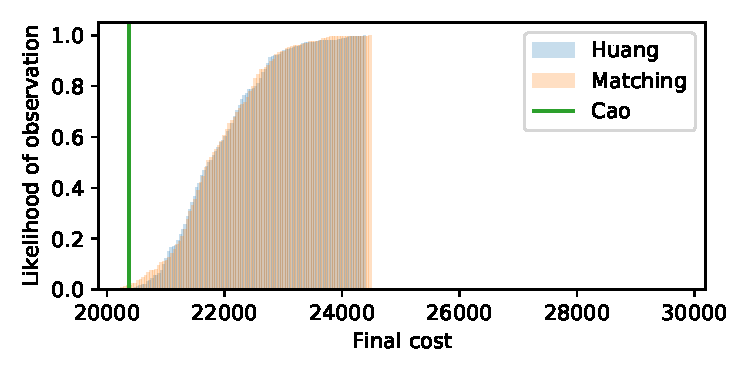
\includegraphics[width=\linewidth]{Fig2b2.pdf}
        \caption{Empirical CDF plots for initial (top) and final (bottom)
                 costs.}
    \end{subfigure}
    \caption{Summative plots for the mushroom dataset with \(k=17\).}%
    \label{fig:mushroom_knee}
\end{figure}

\begin{figure}
    \begin{subfigure}{.5\textwidth}
        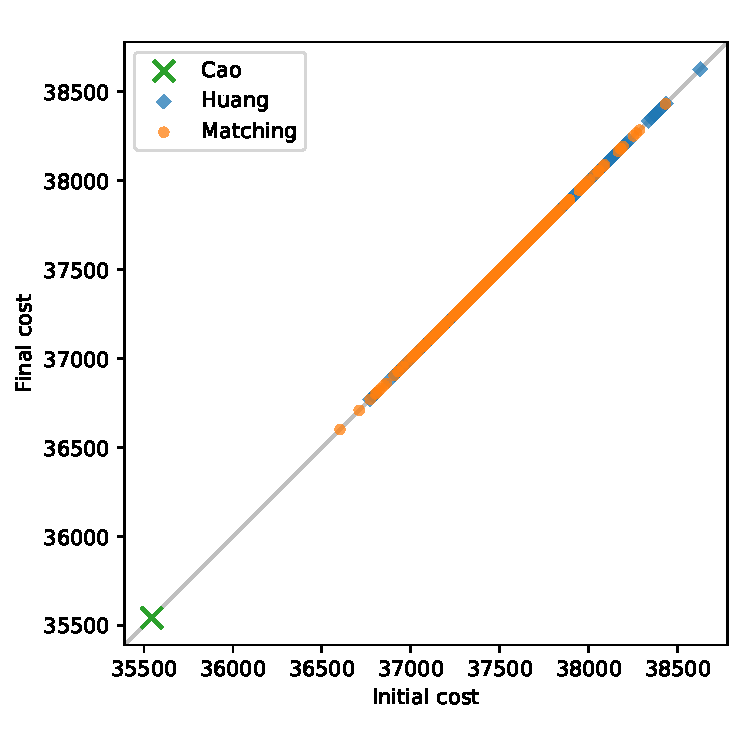
\includegraphics[width=\linewidth]{Fig3a.pdf}
        \caption{Scatter plot of initial and final costs.}
    \end{subfigure}
    \hfill%
    \begin{subfigure}{.5\textwidth}
        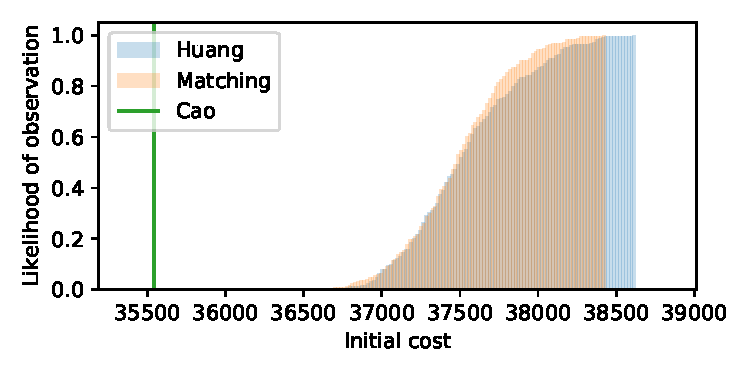
\includegraphics[width=\linewidth]{Fig3b1.pdf}

        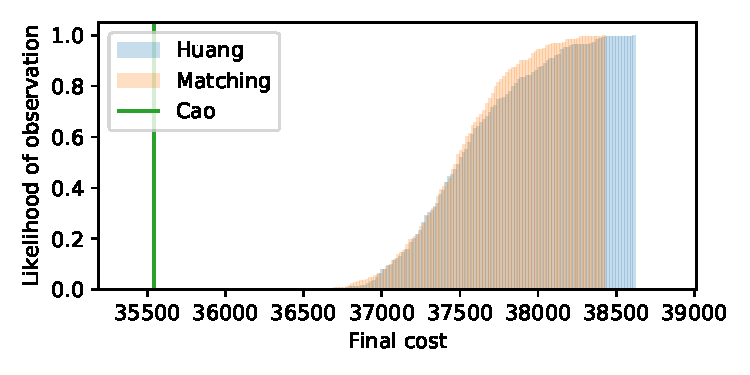
\includegraphics[width=\linewidth]{Fig3b2.pdf}
        \caption{Empirical CDF plots for initial (top) and final (bottom)
                 costs.}
    \end{subfigure}
    \caption{Summative plots for the nursery dataset with \(k=23\).}%
    \label{fig:nursery_knee}
\end{figure}

\begin{figure}
    \begin{subfigure}{.5\textwidth}
        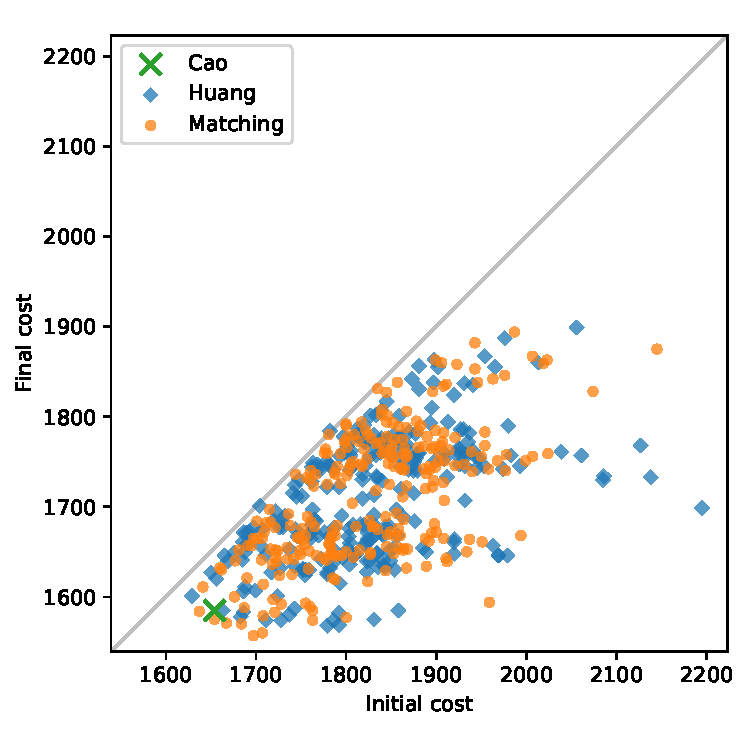
\includegraphics[width=\linewidth]{Fig4a.pdf}
        \caption{Scatter plot of initial and final costs.}
    \end{subfigure}
    \hfill%
    \begin{subfigure}{.5\textwidth}
        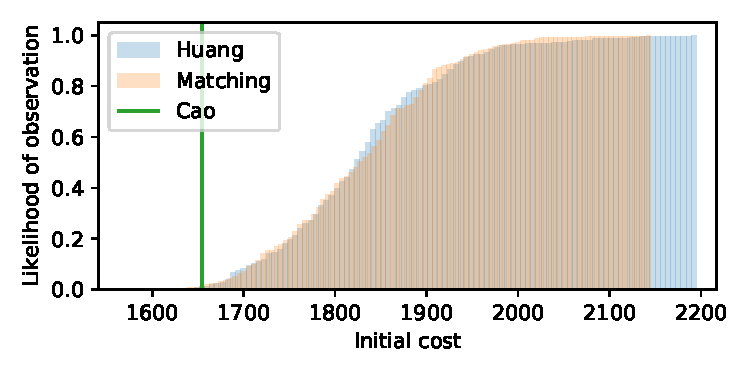
\includegraphics[width=\linewidth]{Fig4b1.pdf}

        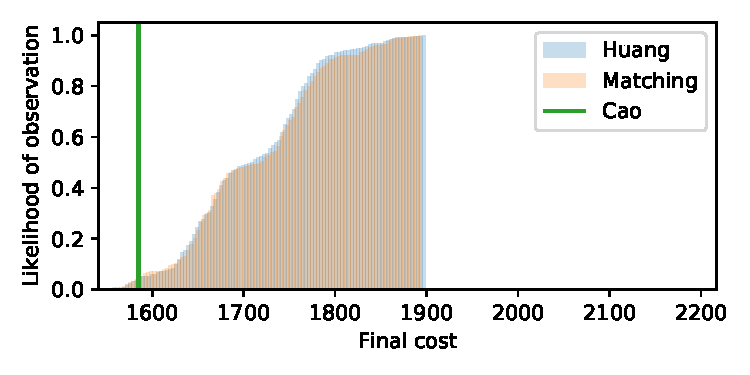
\includegraphics[width=\linewidth]{Fig4b2.pdf}
        \caption{Empirical CDF plots for initial (top) and final (bottom)
                 costs.}
    \end{subfigure}
    \caption{Summative plots for the soybean dataset with \(k=8\).}%
    \label{fig:soybean_knee}
\end{figure}


\subsection{Using number of classes for \(k\)}\label{subsec:nclasses}

As is discussed above, the often automatic choice for \(k\) is the number of
classes present in the data; this subsection repeats the analysis from the
subsection above but with this traditional choice for \(k\).
Tables~\ref{tab:breast_cancer_nclasses}---\ref{tab:soybean_nclasses}
contain the analogous summaries of each initialisation method's performance on
the benchmark datasets over the same number of repetitions.

\begin{table}[htbp]
    \centering
    \resizebox{\tablewidth}{!}{%
        \begin{tabular}{lllll}
\toprule
{} &       Initial cost &         Final cost & No. iterations &          Time \\
\midrule
Cao      &    3315.00 (0.000) &    3172.00 (0.000) &   2.00 (0.000) &  0.13 (0.005) \\
Huang    &  3393.80 (120.772) &  3348.51 (144.849) &   1.54 (0.653) &  0.10 (0.024) \\
Matching &  3406.73 (111.686) &  3355.56 (144.621) &   1.61 (0.638) &  0.09 (0.018) \\
\bottomrule
\end{tabular}

    }
    \captionof{table}{Summative metric results for the breast cancer dataset
    with \(k=2\).}\label{tab:breast_cancer_nclasses}\vspace{20pt}

    \resizebox{\tablewidth}{!}{%
        \begin{tabular}{lllll}
\toprule
{} &         Initial cost &           Final cost & No. iterations &          Time \\
\midrule
Cao      &     37662.00 (0.000) &     37662.00 (0.000) &   1.00 (0.000) &  1.10 (0.142) \\
Huang    &  41720.20 (2519.647) &  38612.64 (2086.246) &   3.14 (1.471) &  2.04 (0.759) \\
Matching &  42297.98 (2265.532) &  39496.56 (2681.581) &   3.36 (1.439) &  1.62 (0.567) \\
\bottomrule
\end{tabular}

    }
    \captionof{table}{Summative metric results for the mushroom dataset with
    \(k=2\).}\label{tab:mushroom_nclasses}\vspace{20pt}

    \resizebox{\tablewidth}{!}{%
        \begin{tabular}{lllll}
\toprule
{} &        Initial cost &          Final cost & No. iterations &          Time \\
\midrule
Cao      &    49060.00 (0.000) &    49060.00 (0.000) &   1.00 (0.000) &  1.80 (0.090) \\
Huang    &  51229.45 (902.503) &  51229.45 (902.503) &   1.00 (0.000) &  1.72 (0.116) \\
Matching &  51107.52 (910.258) &  51101.95 (903.525) &   1.00 (0.063) &  1.37 (0.128) \\
\bottomrule
\end{tabular}

    }
    \captionof{table}{Summative metric results for the nursery dataset with
    \(k=5\).}\label{tab:nursery_nclasses}\vspace{20pt}

    \resizebox{\tablewidth}{!}{%
        \begin{tabular}{lllll}
\toprule
{} &      Initial cost &        Final cost & No. iterations &          Time \\
\midrule
Cao      &   1364.00 (0.000) &   1314.00 (0.000) &   2.00 (0.000) &  0.35 (0.043) \\
Huang    &  1586.90 (83.851) &  1444.56 (58.788) &   4.03 (1.114) &  0.46 (0.085) \\
Matching &  1585.66 (88.345) &  1447.63 (59.620) &   4.04 (1.123) &  0.24 (0.022) \\
\bottomrule
\end{tabular}

    }
    \captionof{table}{Summative metric results for the soybean dataset with
    \(k=15\).}\label{tab:soybean_nclasses}
\end{table}

An immediate comparison to the previous tables is that for all datasets bar the
soybean dataset, the mean costs are significantly higher and the computation
times are lower. These effects come directly from the choice of \(k\) in that
higher values of \(k\) will require more checks (and thus computational time)
but will typically lead to more homogeneous clusters, reducing their
within-cluster dissimilarity and therefore cost.

Looking at these tables on their own, Cao's method is the superior
initialisation method on average: the means are substantially lower in terms of
initial and final cost; there is no deviation in these results; again, the total
computational time is a fraction of the other two methods. It is also apparent
that Huang's method and the proposed extension are very comparable on average.
As before, finer investigation will require finer visualisations.
Figures~\ref{fig:breast_cancer_nclasses}---\ref{fig:soybean_nclasses} show the
same plots as in the previous subsection except the number of clusters has been
taken to be the number of classes present in each dataset.

Figures~\ref{fig:breast_cancer_nclasses}~\&~\ref{fig:mushroom_nclasses} indicate
that a particular behaviour emerged during the runs of the \(k\)-modes
algorithm. Specifically, each solution falls into one of (predominantly) two
types: effectively no improvement on the initial clustering, or terminating at
some clustering with a cost that is bounded below across all such solutions.
Invariably, Cao's method achieves or approaches this lower bound and unless
Cao's method is used, these particular choices for \(k\) mean that the
performance of the \(k\)-modes algorithm is exceptionally sensitive to its
initial clustering. Moreover, the other two methods are effectively
indistinguishable in these cases and so if a robust solution is required, Cao's
method is the only viable option.

Figure~\ref{fig:nursery_nclasses} corresponds to the nursery dataset results
with \(k=5\). In this set of runs, the same pattern emerges as in
Figure~\ref{fig:nursery_knee} where sampling the initial centres from amongst
the most dense points (via Huang's method and the proposed) is an inferior
strategy to one considering the entire attribute space such as with Cao's
method. Again, no method is able to improve on the initial solution except for
one repetition with the matching initialisation method.

\begin{figure}
    \begin{subfigure}{.5\textwidth}
        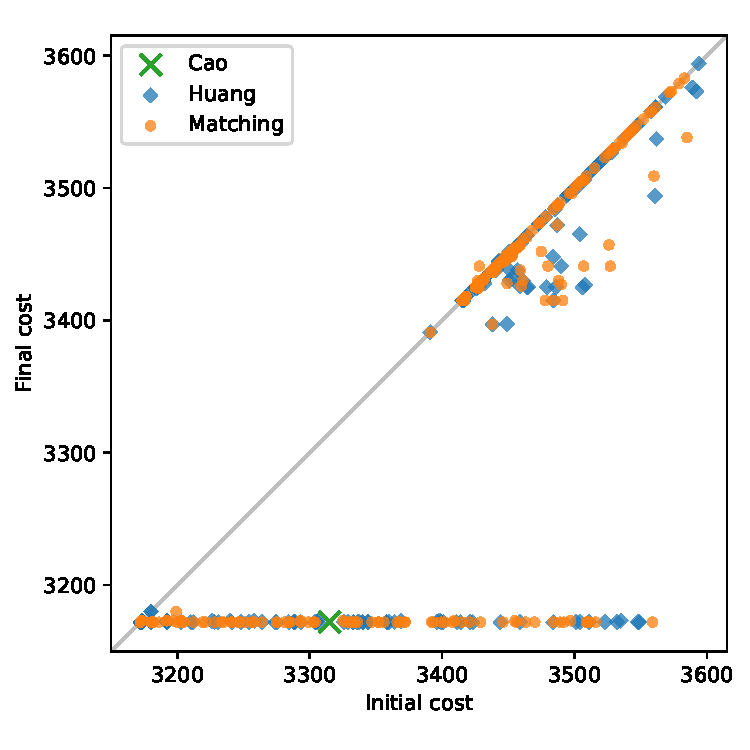
\includegraphics[width=\linewidth]{Fig5a.pdf}
        \caption{Scatter plot of initial and final costs.}
    \end{subfigure}
    \hfill%
    \begin{subfigure}{.5\textwidth}
        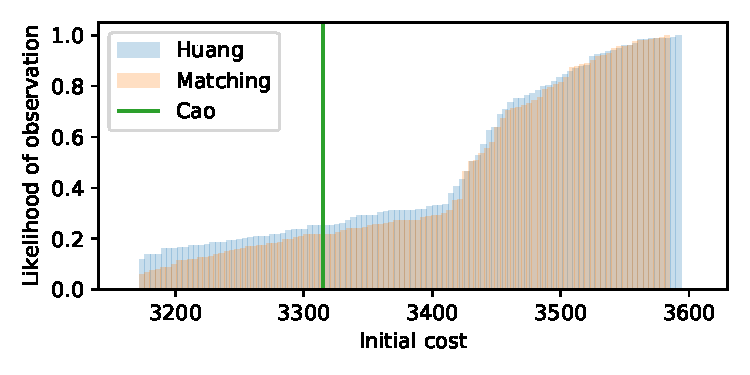
\includegraphics[width=\linewidth]{Fig5b1.pdf}

        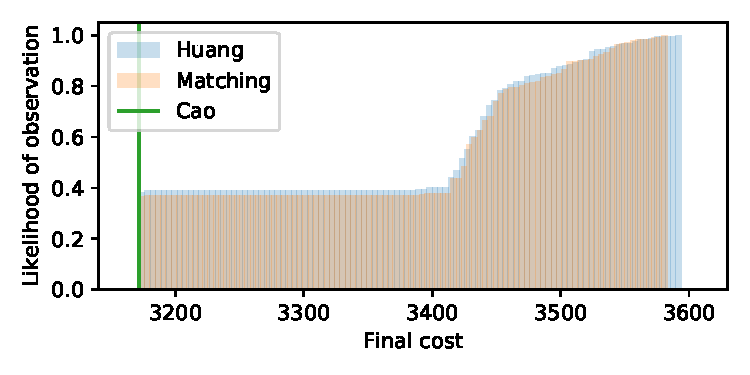
\includegraphics[width=\linewidth]{Fig5b2.pdf}
        \caption{Empirical CDF plots for initial (top) and final (bottom)
                 costs.}
    \end{subfigure}
    \caption{Summative plots for the breast cancer dataset with \(k=2\).}%
    \label{fig:breast_cancer_nclasses}
\end{figure}

\begin{figure}
    \begin{subfigure}{.5\textwidth}
        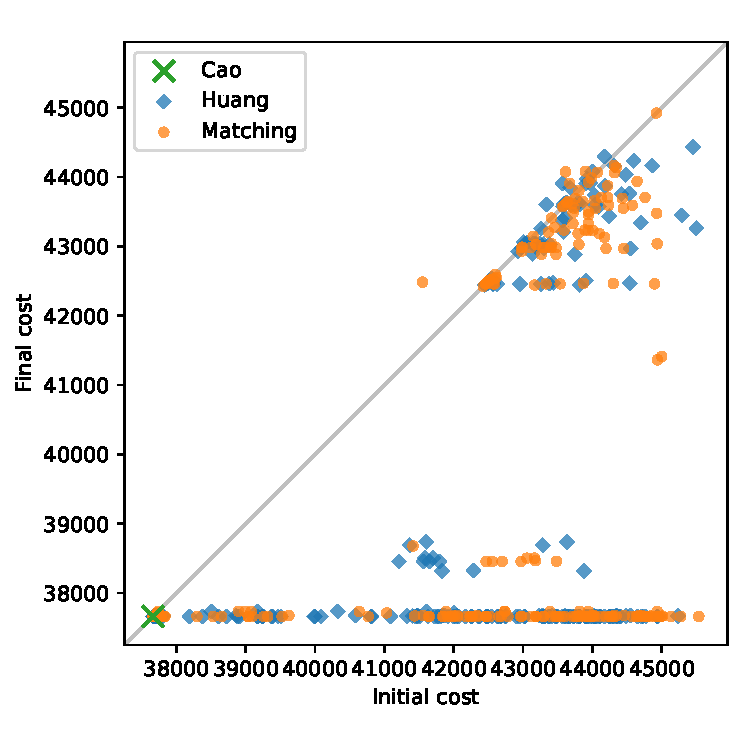
\includegraphics[width=\linewidth]{Fig6a.pdf}
        \caption{Scatter plot of initial and final costs.}
    \end{subfigure}
    \hfill%
    \begin{subfigure}{.5\textwidth}
        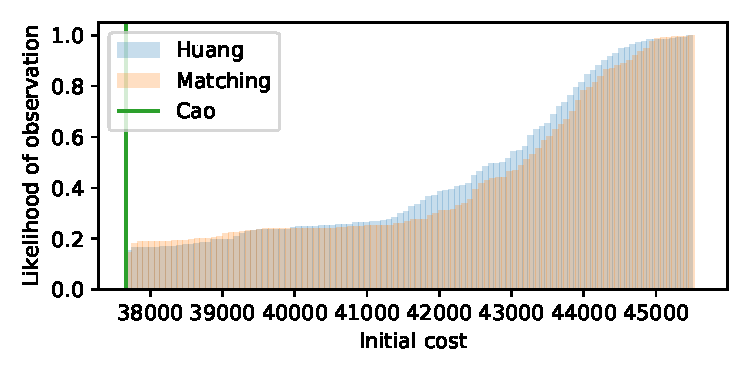
\includegraphics[width=\linewidth]{Fig6b1.pdf}

        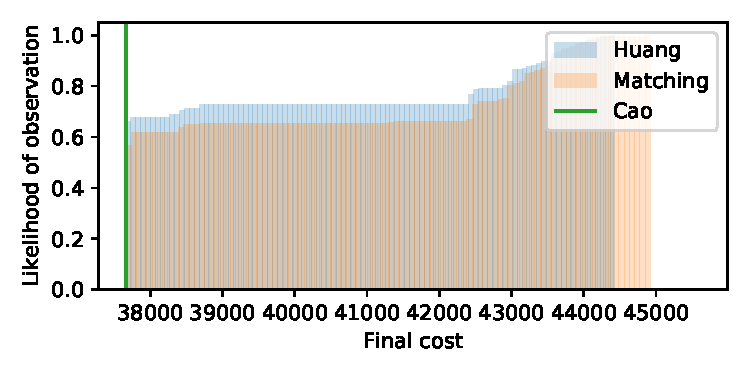
\includegraphics[width=\linewidth]{Fig6b2.pdf}
        \caption{Empirical CDF plots for initial (top) and final (bottom)
                 costs.}
    \end{subfigure}
    \caption{Summative plots for the mushroom dataset with \(k=2\).}%
    \label{fig:mushroom_nclasses}
\end{figure}

\begin{figure}
    \begin{subfigure}{.5\textwidth}
        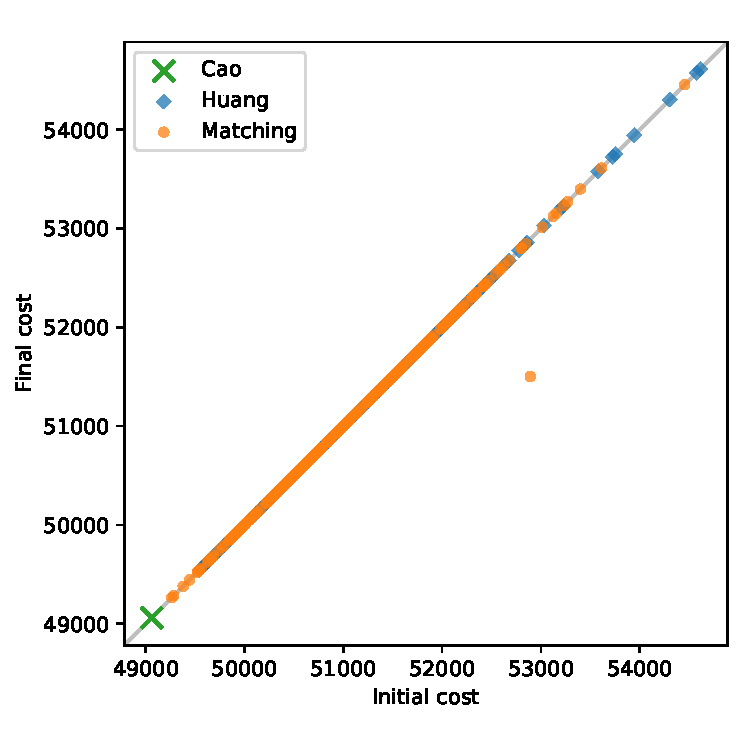
\includegraphics[width=\linewidth]{Fig7a.pdf}
        \caption{Scatter plot of initial and final costs.}
    \end{subfigure}
    \hfill%
    \begin{subfigure}{.5\textwidth}
        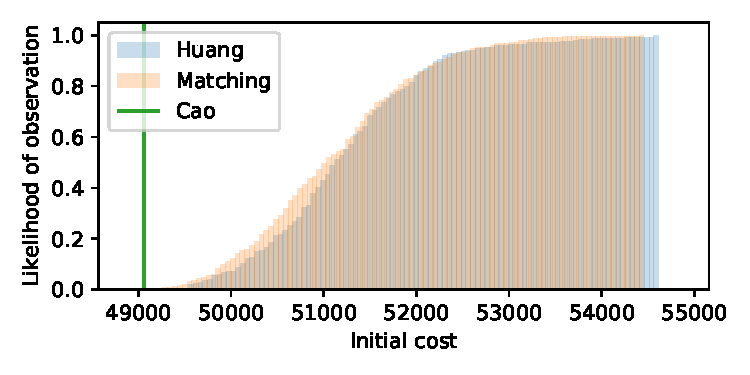
\includegraphics[width=\linewidth]{Fig7b1.pdf}

        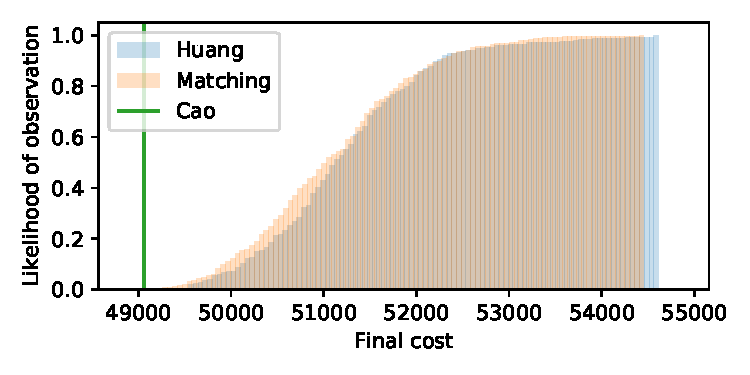
\includegraphics[width=\linewidth]{Fig7b2.pdf}
        \caption{Empirical CDF plots for initial (top) and final (bottom)
                 costs.}
    \end{subfigure}
    \caption{Summative plots for the nursery dataset with \(k=5\).}%
    \label{fig:nursery_nclasses}
\end{figure}

\begin{figure}
    \begin{subfigure}{.5\textwidth}
        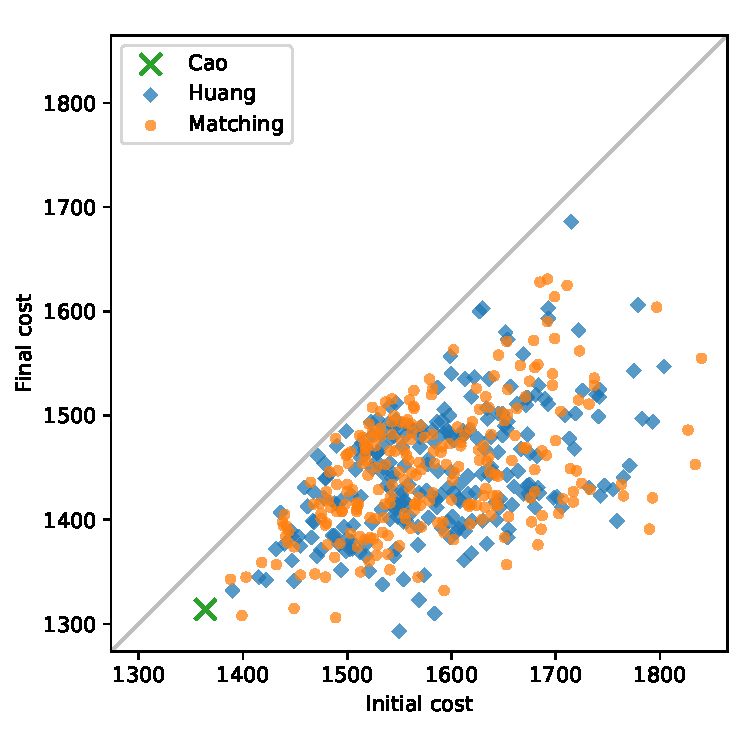
\includegraphics[width=\linewidth]{Fig8a.pdf}
        \caption{Scatter plot of initial and final costs.}
    \end{subfigure}
    \hfill%
    \begin{subfigure}{.5\textwidth}
        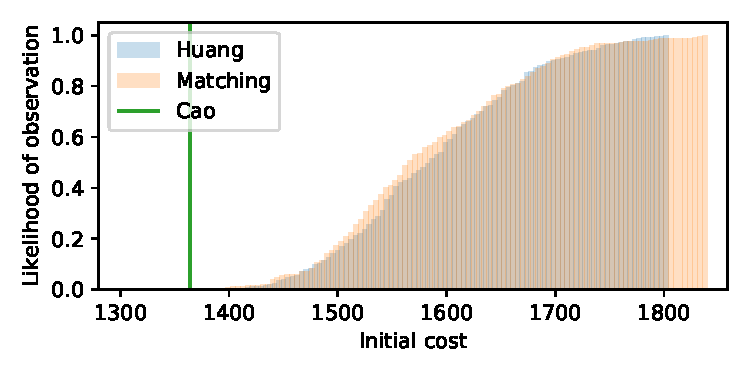
\includegraphics[width=\linewidth]{Fig8b1.pdf}

        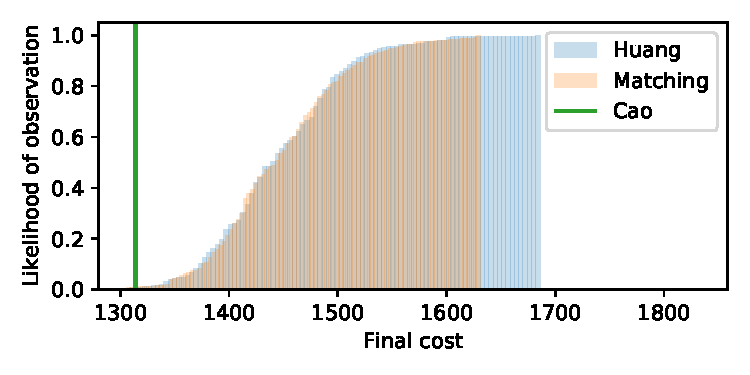
\includegraphics[width=\linewidth]{Fig8b2.pdf}
        \caption{Empirical CDF plots for initial (top) and final (bottom)
                 costs.}
    \end{subfigure}
    \caption{Summative plots for the soybean dataset with \(k=15\).}%
    \label{fig:soybean_nclasses}
\end{figure}

The primary conclusion from this analysis is that while Huang's method is
largely comparable to the proposed extension, there is no substantial evidence
from these use cases to use Huang's method over the one proposed in this work.
In fact, Figure~\ref{fig:soybean_nclasses} is the only instance where Huang's
method was able to outperform the proposed method. Other than this, the proposed
method consistently performing better (or as well as) Huang's method in terms of
minimal final costs and computational time over a number of runs in both the
cases where an external framework is imposed on the data (by choosing \(k\) to
be the number of classes) and not. Furthermore, though not discussed in this
work, the matching initialisation method has the scope to allow for expert or
prior knowledge to be included in an initial clustering by using some \textit{ad
hoc} preference list mechanism.


\subsection{Artificial datasets}\label{subsec:artificial}

Following on from the conclusions of the analysis thus far, the competition
between Cao's method and the proposed matching method may be studied more
deeply. All of the results leading up to this point were conducted using
benchmark datasets and while there are certainly benefits to comparing methods
in this way, it does not afford a rich understanding of how any of them perform
more generally. This stage of the analysis relies on a method for generating
artificial datasets introduced in~\cite{Wilde2019}. In essence, this method is
an evolutionary algorithm which acts on entire datasets to explore the space in
which potentially all possible datasets exist. The key component of this method
is an objective function that takes a dataset and returns a value that is to be
minimised; this function is referred to as the fitness function.

In order to reveal the nuances in the performance of Cao's method and the
proposed initialisation on a particular dataset, two cases are considered:
where Cao's method outperforms the proposed, and vice versa. Both cases use the
same fitness function --- with the latter using its negative --- which is
defined as follows:
\begin{equation}\label{eq:fitness}
    f\left(\mathcal X\right) = C_{\mathrm{cao}} - C_{\mathrm{match}}
\end{equation}
where \(C_{\mathrm{cao}}\) and \(C_{\mathrm{match}}\) are the final costs when a
dataset \(\mathcal X\) is clustered using Cao's method and the proposed matching
method respectively with \(k = 3\). For the sake of computational time, the
proposed initialisation was given 25 repetitions as opposed to the 250
repetitions in the remainder of this section. Apart from the sign of \(f\), the
dataset generation processes used identical parameters in each case and the
datasets considered here are all of comparable shape.

\begin{figure}
    \centering
    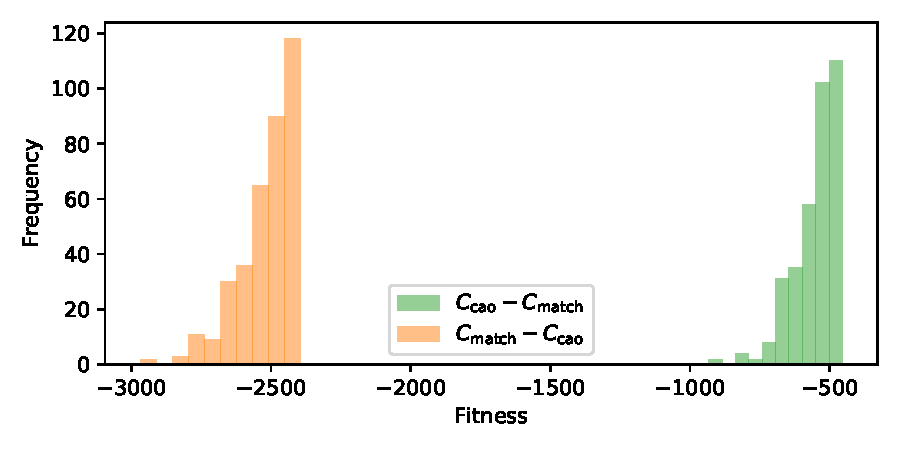
\includegraphics[width=\imgwidth]{Fig9.pdf}
    \caption{Histograms of fitness for the top performing percentile in each
             case.}\label{fig:fitness}
\end{figure}

This process yielded approximately 35,000 unique datasets for each case, and the
ensuing analysis only considers the top-performing percentile of datasets from
each. Figure~\ref{fig:fitness} shows the fitness distribution of the top
percentile in each case. It should be clear from~\eqref{eq:fitness} that large
negative values are preferable here. With that, and bearing in mind that the
generation of these datasets was parameterised in a consistent manner, it
appears that the attempt to outperform Cao's method proved somewhat easier. This
is indicated by the substantial difference in the locations of the fitness
distributions.

Given the quantity of data available, to understand the patterns that have
emerged, they must be summarised; in this case, univariate statistics are used.
Despite the datasets all being of similar shapes, there are some discrepancies.
With the number of rows this is less of an issue but any comparison of
statistics across datasets of different widths is difficult without prior
knowledge of the datasets. Moreover, there is no guarantee of contingency
amongst the attributes, and the comparison of more than a handful of variables
becomes complicated even when the attributes are identifiable. To combat this
and bring uniformity to the datasets, each dataset is represented as their first
principal component obtained via centred Principal Component Analysis
(PCA)~\cite{Jolliffe1986}. While some subtleties may be lost, this
representation captures the most important characteristics of each dataset in a
single variable meaning they can be compared directly.

Since the transformation by PCA is centred, all measures for central tendency
are moot. In fact, the mean and median are not interpretable here given that the
original data is categorical. As such, the univariate statistics used here
describe the spread and shape of the principal components, and are split into
two groups:
\begin{itemize}
    \item Central moments: variance, skewness and kurtosis.
    \item Empirical quantiles: interquartile range, lower decile and upper
        decile.
\end{itemize}

Figures~\ref{fig:edo_moments}~\&~\ref{fig:edo_quantiles} show the distributions
of the six univariate statistics across all of the principal components in each
case. In addition to this, they show a fitted Gaussian kernel density
estimate~\cite{Bashtannyk2001} to accentuate the general shape of the
histograms. What becomes immediately clear from each of these plots is that for
datasets where Cao's method succeeds, the general spread of their first
principal component is much tighter than in the case where the proposed
initialisation method succeeds. This is particularly evident in
Figure~\ref{fig:edo_variance} where relatively low variance in the first case
indicates a higher level of density in the original categorical data.

The patterns in the quantiles further this. Although Figure~\ref{fig:edo_iqr}
suggests that the components of Cao-preferable datasets can have higher
interquartile ranges than in the second case, the lower and upper deciles tend
to be closer together as is seen in
Figures~\ref{fig:edo_lower}~\&~\ref{fig:edo_upper}. This suggests that despite
the body of the component being spread, its extremities are not.

In Figures~\ref{fig:edo_skewness}~\&~\ref{fig:edo_kurtosis}, the most notable
contrast between the two cases is the range in values for both skewness and
kurtosis. This supports the evidence thus far that individual datasets have
higher densities and lower variety (i.e.\ tighter extremities) when Cao's method
succeeds over the proposed initialisation. In particular, larger values of
skewness and kurtosis translate to high similarity between the instances in a
categorical dataset which is equivalent to having high density.

Overall, this analysis has revealed that if a dataset shows clear evidence of
high-density points, then Cao's method should be used over the proposed method.
However, if there is no such evidence, the proposed method is able to find a
substantially better clustering than Cao's method.

\begin{figure}
    \centering
    \begin{subfigure}{\imgwidth}
        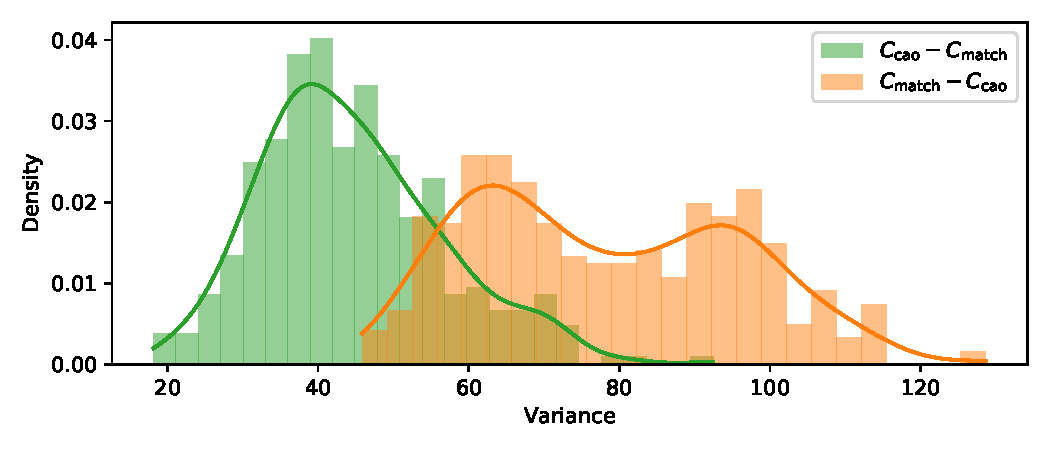
\includegraphics[width=\linewidth]{Fig10a.pdf}%
        \caption{}\label{fig:edo_variance}
    \end{subfigure}

    \begin{subfigure}{\imgwidth}
        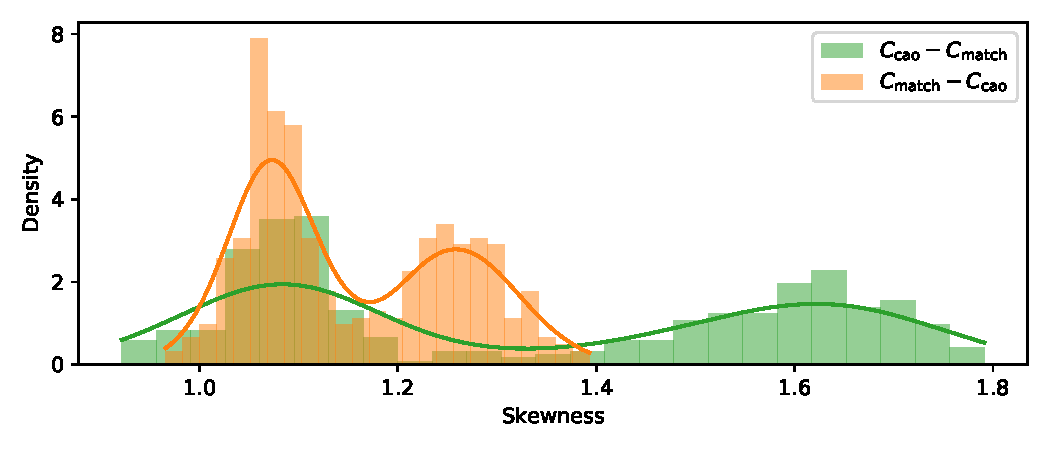
\includegraphics[width=\linewidth]{Fig10b.pdf}%
    \caption{}\label{fig:edo_skewness}
    \end{subfigure}
    
    \begin{subfigure}{\imgwidth}
        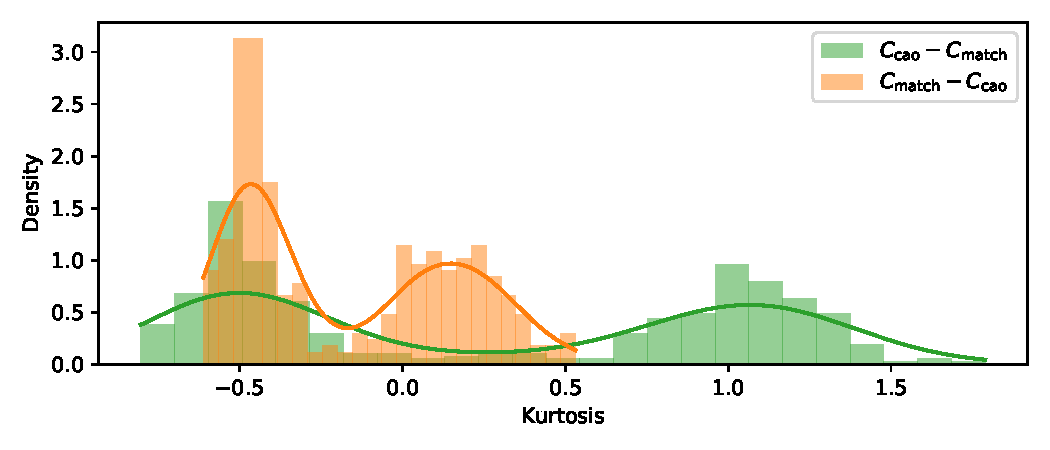
\includegraphics[width=\linewidth]{Fig10c.pdf}%
        \caption{}\label{fig:edo_kurtosis}
    \end{subfigure}
    \caption{Distribution plots for the (\subref{fig:edo_variance}) variance,
        (\subref{fig:edo_skewness}) skewness and (\subref{fig:edo_kurtosis})
        kurtosis of the first principal components in each
        case.}\label{fig:edo_moments}
\end{figure}

\begin{figure}
    \centering
    \begin{subfigure}{\imgwidth}
        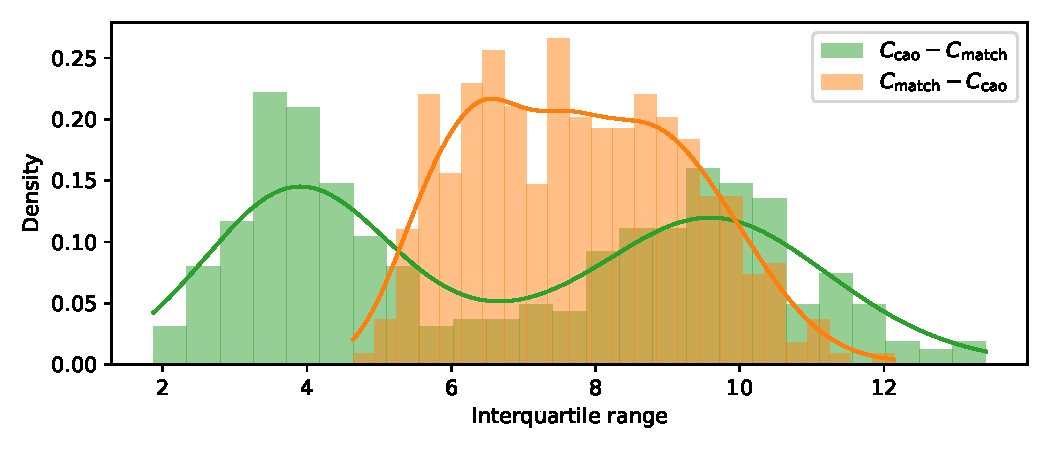
\includegraphics[width=\linewidth]{Fig11a.pdf}
        \caption{}\label{fig:edo_iqr}
    \end{subfigure}\vfill%

    \begin{subfigure}{\imgwidth}
        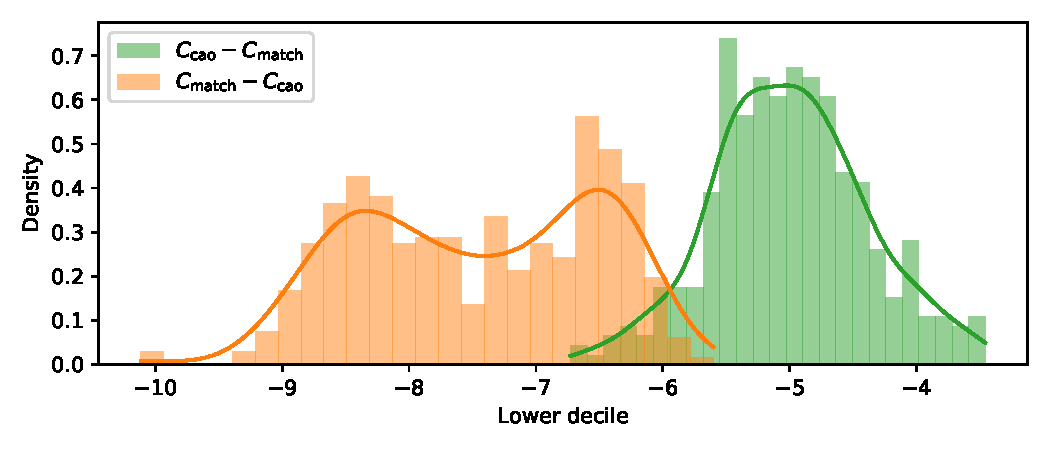
\includegraphics[width=\linewidth]{Fig11b.pdf}
        \caption{}\label{fig:edo_lower}
    \end{subfigure}\vfill%
    
    \begin{subfigure}{\imgwidth}
        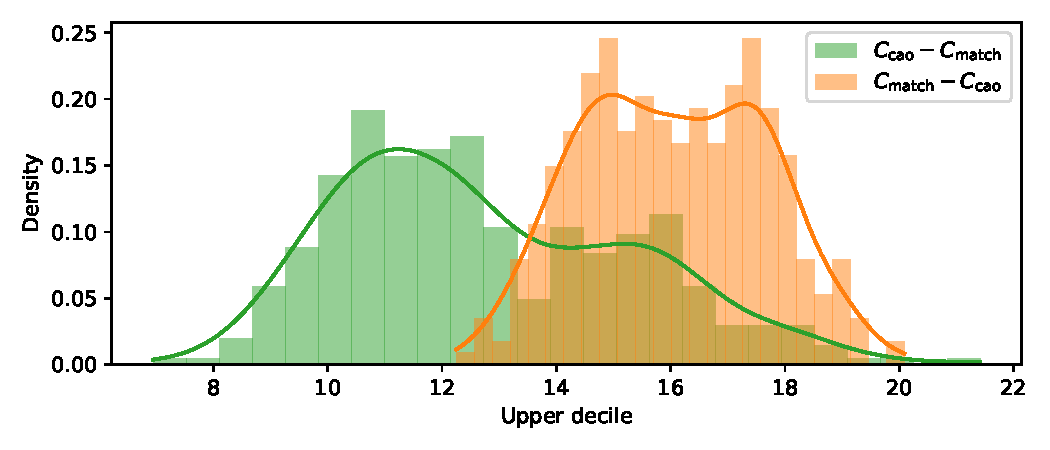
\includegraphics[width=\linewidth]{Fig11c.pdf}
        \caption{}\label{fig:edo_upper}
    \end{subfigure}
    \caption{Distribution plots for the (\subref{fig:edo_iqr}) interquartile
        range, (\subref{fig:edo_lower}) lower decile and
        (\subref{fig:edo_upper}) upper decile of the first principal components
        in each case.}\label{fig:edo_quantiles}
\end{figure}


